\section{Solutions for The Experiments of Conceptual Clustering}
\subsection{Solution for Experiment 1}
The tree generated for the input sequence 1 and sequence 2 are shown in the following:
\begin{figure}[h!]
    \centering
    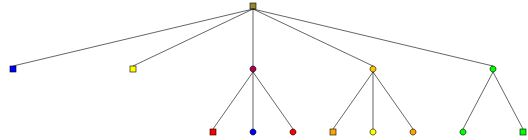
\includegraphics[width=300pt]{../images/experiment1_seq1_9.jpg}
    \caption{Experiment 1 with sequence 1}
    \label{Fig:experiment1_seq1}
\end{figure}

\begin{figure}[h!]
    \centering
    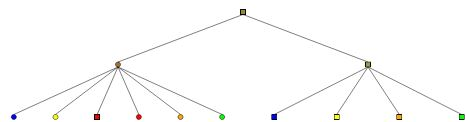
\includegraphics[width=300pt]{../images/experiment1_seq2_9.jpg}
    \caption{Experiment 1 with sequence 2}
    \label{Fig:experiment1_seq2}
\end{figure}

\subsection{Solution for Experiment 2}
Answers for this experiment are open. Here is one possible example. In an organization, people are grouped to different departments. Whenever new people come in, it will be decided which department they should join. Sometimes, several departments are merged to one and in some cases, one department might be broken down into several because of the newly added people. Attributes and values for this specific example could be:\\
\emph{experience,preference,age,gender,advantage\#\\
 extensive,relevant,none\#\\
 sales,management,logistics,nopreference\#\\
 female,male\#\\
 under,twenties,thirties,forties,above\#\\
 design,writing,communication\#\\} 

\subsection{Solution for Experiment 3}
There are usually three key steps to get the category utility of a certain classification. First, get the probability of each class. It is very straightforward. You just need to calculate the fraction of the number of objects in a certain class against the total number of objects. In this exercise, the number of objects in \emph{Class 1} is three, the same for \emph{class 2} and the total number of objects is six. Thus, the probability for $C_1$ is $$P(C_1)=\frac{3}{6}=0.5$$ and the probability for $C_2$ is $$P(C_2)=\frac{3}{6}=0.5$$ 

Second, get the expected number of attribute values that can be correctly guessed given a certain class. This is the conditional expectations (See Page 5). For each attribute value given \emph{Class 1}, we can get the following table \ref{tab:solexperiment3}:

\begin{table}[!ht]
 \ttabbox{\caption{}}
 {
 \centering
 \begin{tabular}{l l l l l l}\hline
 \textbf{ } & \textbf{ } & \textbf{Class 1 } & \textbf{} & \textbf{ } & \textbf{ } \\
 \textbf{A1} & \textbf{ } & \textbf{A2} & \textbf{ } & \textbf{A3} & \textbf{ } \\\hline
 \textbf{Green} & $({2}/{3})^2$ & \textbf{Ball} & $({3}/{3})^2$ & \textbf{Small} & $({2}/{3})^2$ \\
 \textbf{Red} & $({1}/{3})^2$ & \textbf{Square} & $(0/3)^2$ & \textbf{Large} & $({1}/{3})^2$ \\
 \textbf{Blue} & $(0/3)^2$ & -- & -- & -- & -- \\\hline
 \end{tabular}
 \label{tab:solexperiment3}}
 \end{table}
 The expected number of attribute values that can be correctly guessed given $C_1$ is: $$\sum_{i=1}^{3} \sum_{j=1}^{}P(A_i=V_{ij}\left|C_1\right.)^2=(\frac{2}{3})^2+(\frac{1}{3})^2+0+1+0+(\frac{2}{3})^2+(\frac{1}{3})^2=2.11$$
 
For each attribute value given \emph{Class 2}, we can get the following table \ref{tab:solexperiment31}:
  
  \begin{table}[!ht]
   \ttabbox{\caption{}}
   {
   \centering
   \begin{tabular}{l l l l l l}\hline
   \textbf{ } & \textbf{ } & \textbf{Class 1 } & \textbf{} & \textbf{ } & \textbf{ } \\
   \textbf{A1} & \textbf{ } & \textbf{A2} & \textbf{ } & \textbf{A3} & \textbf{ } \\\hline
   \textbf{Green} & $({1}/{3})^2$ & \textbf{Ball} & $({1}/{3})^2$ & \textbf{Small} & $({0}/{3})^2$ \\
   \textbf{Red} & $({0}/{3})^2$ & \textbf{Square} & $(2/3)^2$ & \textbf{Large} & $({3}/{3})^2$ \\
   \textbf{Blue} & $(2/3)^2$ & -- & -- & -- & -- \\\hline
   \end{tabular}
   \label{tab:solexperiment31}}
   \end{table}
The expected number of attribute values that can be correctly guessed given $C_2$ is: $$\sum_{i=1}^{3} \sum_{j=1}^{}P(A_i=V_{ij}\left|C_2\right.)^2=(\frac{1}{3})^2+0+(\frac{2}{3})^2+(\frac{1}{3})^2+(\frac{2}{3})^2+0+1=2.11$$

Last, get the expected number of attribute values that can be correctly guessed without any category knowledge. This is the unconditional expectations.
 \begin{table}[!ht]
   \ttabbox{\caption{}}
   {
   \centering
   \begin{tabular}{l l l l l l}\hline
   \textbf{A1} & \textbf{ } & \textbf{A2} & \textbf{ } & \textbf{A3} & \textbf{ } \\\hline
   \textbf{Green} & $({3}/{6})^2$ & \textbf{Ball} & $({4}/{6})^2$ & \textbf{Small} & $(2/6)^2$ \\
   \textbf{Red} & $(1/6)^2$ & \textbf{Square} & $(2/6)^2$ & \textbf{Large} & $(4/6)^2$ \\
   \textbf{Blue} & $(2/6)^2$ & -- & -- & -- & -- \\\hline
   \end{tabular}
   \label{tab:solexperiment32}}
   \end{table}
   
The expected number of attribute values that can be correctly guessed without any category information is: $$\sum_{i=1}^{3} \sum_{j=1}^{}P(A_i=V_{ij})^2=(\frac{3}{6})^2+(\frac{1}{6})^2+(\frac{2}{6})^2+(\frac{4}{6})^2+(\frac{2}{6})^2+(\frac{2}{6})^2+(\frac{4}{6})^2=1.5$$
Thus, we can get Category Utility for the current classification: $$CU=\frac{0.5\times(2.11-1.50)+0.5\times(2.11-1.50)}{2}=0.305$$

\subsection {Solution for Experiment 4}
If we go to the function \emph{undoLastStep()} in the file \emph{cluster.js}, we can see that there are four variables that hold the string representation of the cluster. These four variables are \emph{global\_backup\_text1, global\_backup\_text2, global\_backup\_text3 and global\_backup\_text4}. If you search any of them, you will see that they are defined in the very beginning of the \emph{cluster.js}. 

In order to see how the initial value is passed to the \emph{global\_backup\_text}, we need to search the first variable \emph{global\_backup\_text1}. Then you will find out that variable \emph{global\_backup\_text1} gets sting in the function \emph{addObjects()} and function \emph{addRandomObjects()}. Once the variable \emph{global\_backup\_text1} is updated, its previous string will be passed to the variable \emph{global\_backup\_text2} and so on so forth.

Then we go back to the function \emph{undoLastStep()} and now it is easy to know that if we want to undo the last step, we need to recover the values for the variables \emph{global\_backup\_text}. If we want to undo five steps, a new variable \emph{global\_backup\_text5} needs adding in this file. In order to solve this problem, there are four places that needs modifying in \emph{cluster.js}.
\begin{enumerate}[1)]
\item Add \emph{var global\_backup\_text5 = \lq\lq \rq\rq;} in the very beginning of \emph{cluster.js} to define it;
\item Add \emph{global\_backup\_text5 = global\_backup\_text4;} before the code \emph{global\_backup\_text4 = global\_backup\_text3;} in the beginning of the function \emph{addObjects()} to make sure that \emph{global\_backup\_text5} gets the value; 
\item Similar to the second. Add \emph{global\_backup\_text5 = global\_backup\_text4;} before the code \emph{global\_backup\_text4 = global\_backup\_text3;} in the middle of the function \emph{addRandomObjects()};
\item The last place that needs modifying is in the function \emph{undoLastStep()}. In the \emph{else} clause, add \emph{global\_backup\_text4 = global\_backup\_text5;} in front of the code \emph{global\_backup\_text4 = \lq\lq \rq\rq;} and change the code \emph{global\_backup\_text4 = \lq\lq \rq\rq;} to be \emph{global\_backup\_text5= \lq\lq \rq\rq;}
\item Restart the Conceptual Clustering simulation tool and the use the default setting. Add the objects more than five times and then try \lq\lq Undo Last Action \rq\rq button. You will be allowd to undo the last five steps instead of four.
\end{enumerate}